\documentclass[10pt]{beamer}
\usepackage[absolute,overlay]{textpos}
%\usepackage[pdftex]{graphicx}
\usepackage{alltt}
%\usepackage[margin=1in]{geometry}
\usepackage{amsmath, amsthm, amssymb}
\usepackage{verbatim}
\usepackage{ragged2e}
\usepackage{enumitem}
\usepackage{xfrac}
\setlist{parsep=0pt,listparindent=\parindent}
\setlength{\RaggedRightParindent}{\parindent}
\newcommand{\degree}{\ensuremath{^\circ}}
\newcommand{\n}{\break}
\usepackage{accents}
\let\thinbar\bar
\newcommand\thickbar[1]{\accentset{\rule{.4em}{.8pt}}{#1}}
\let\bar\thickbar
\usepackage{standalone}
\usepackage{hyperref}
\usepackage{venndiagram}
\usepackage{mathtools}
\usepackage{bm}
\usepackage[mathscr]{eucal}
\usepackage{tabularx}
\newcolumntype{C}{>{\centering\arraybackslash $}X<{$}}
\usepackage{minted} %colored code in slides

\newcommand{\R}{\ensuremath{\mathbb{R}}}
\newcommand{\N}{\ensuremath{\mathbb{N}}}
\newcommand{\card}{\ensuremath{\text{card }}}
\DeclarePairedDelimiter{\ceil}{\lceil}{\rceil}
\DeclarePairedDelimiter{\floor}{\lfloor}{\rfloor}
\DeclarePairedDelimiter\abs{\lvert}{\rvert}
\DeclarePairedDelimiter\norm{\lVert}{\rVert}
\newcommand\inv[1]{\ensuremath{{#1}^{-1}}}
% \newcommand\arrowdef{\ensuremath{\stackrel{\mathclap{\normalfont\mbox{def}}}{\iff}}}
\newcommand\arrowdef{\mathrel{\overset{\makebox[0pt]{\mbox{\normalfont\scriptsize\sffamily def}}}{\iff}}}
\makeatletter
\newcases{dlrcases}{\quad}{%
  $\m@th\displaystyle{##}$\hfil}{$\m@th\displaystyle{##}$\hfil}{\lbrace}{\rbrace}
\newcases{lrcases}{\quad}{%
  $\m@th{##}$\hfil}{{##}\hfil}{\lbrace}{\rbrace}
\makeatother

%%%%%%%%%%%%%%%%%%%%%%%%%%%%%%%%%%%%%%%%%%%%%%%%%%%%%
% graphs/automata
\usepackage{tikz}
\usetikzlibrary{arrows,automata}
\tikzset{myAutomata/.style={
    >=stealth',
    shorten >=1pt,
    auto,
    node distance=2cm,
    accepting/.style={
      double distance=1pt,
      outer sep=0.5pt+\pgflinewidth
    },
    initial text={}
 }}
%%%%%%%%%%%%%%%%%%%%%%%%%%%%%%%%%%%%%%%%%%%%%%%%%%%%%

%%%%%%%%%%%%%%%%%%%%%%%%%%%%%%%%%%%%%%%%%%%%%%%%%%%%%
%beamer only
\title{Game of Life On Compact Topologies}
\subtitle{With a focus on vertical walls on a torus}
\author{Marc Gotliboym}
\date{\today}
\hypersetup{pdfstartview={Fit}} % fits the presentation to the window when first displayed

\newcommand\frametext[1]{%
  \begin{textblock*}{\paperwidth}(0pt,0.6cm)%\textheight)
    \raggedleft #1
  \end{textblock*}}

\setitemize{label=\usebeamerfont*{itemize item}%
  \usebeamercolor[fg]{itemize item}
  \usebeamertemplate{itemize item}}
%%%%%%%%%%%%%%%%%%%%%%%%%%%%%%%%%%%%%%%%%%%%%%%%%%%%%
\begin{document}
\frame{\titlepage}
\begin{frame}
  \frametitle{Game of Life}
  \begin{itemize}
    \item Cellular Automaton
    \item For each cell, living on the next generation iff \\
    it is alive and has 2 or 3 neighors, or it is dead and has 3 neighbors.
  \end{itemize}
  \begin{tabularx}{\textwidth}{@{\rule[-3ex]{0pt}{7ex}}|*{7}{C|}}
    \hline
     &  &  &  &  &  &  \\
    \hline
     &  &  &  &L  &  &  \\
    \hline
     &  &  &L &  &  &  \\
    \hline
     &  &  &  &L &L  &  \\
    \hline
     &  &  &L  &  &  &  \\
    \hline
     &  &  &  &  &  &  \\
    \hline
  \end{tabularx}
\end{frame}

\begin{frame}
  \frametitle{Compact Topologies}
  \begin{columns}
    \begin{column}{0.5\textwidth}
      \begin{itemize}
        \item Klein Bottle
        \item Torus \\
        \item Let's see a glider!
      \end{itemize}
    \end{column}
    \begin{column}{0.5\textwidth}
      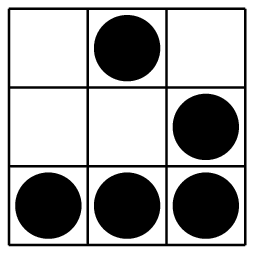
\includegraphics[height=3cm]{glider}
    \end{column}
  \end{columns}
\end{frame}

\begin{frame}[fragile]
  \frametitle{Comonadic Cellular Automaton}
  \begin{minted}{haskell}
square (SpaceZipTorus zs) =
  let (top:mid:bottom:[]) = getRow zs
    in getRow top : getRow mid : getRow bottom : []
  where getRow xs = (focus $ leftMv xs) : (focus xs) :
                      (focus $ rightMv xs) : []
    
gameOfLifeRule :: (SpaceZip p z1 z2) => p z1 z2 Bool -> Bool
gameOfLifeRule s =
  let numNeighbors = sum $ (map fromEnum) $ concat $ square s
    in if (extract s) then numNeighbors==3 || numNeighbors==4 
    else numNeighbors==3

applyRule s = extend gameOfLifeRule s
  \end{minted}
  %$
\end{frame}

\begin{frame}
  \frametitle{Simplifying}
  \begin{itemize}
    \item Start on a torus, and make one vertical line of cells alive.
    \item Sierpinski triangle! (width: 63)
    \item What happens every $2^n$ steps?
  \end{itemize}
\end{frame}

\begin{frame}
  \frametitle{Fuses and Cycles}
  \begin{itemize}
    \item Every board has to cycle eventually.
    \item It need not cycle back to the start --- fuse.
    \item See width 23
  \end{itemize}
\end{frame}

\begin{frame}[fragile]
  \frametitle{Patterns in fuses}
  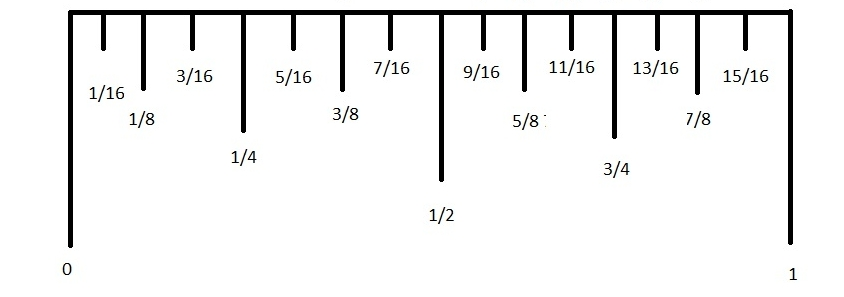
\includegraphics[height=3cm]{ruler}
  \begin{itemize}
    \item abacabadabacaba
    \item The fuses for boards with widths which are 3 modulo 4 are:
  \end{itemize}
\begin{verbatim}
                                     0
                   2                 0                        
                 2 4  2              0
             2 4 2 8  2 4 2          0
     2 4 2 8 2 4 2 16 2 4 2 8 2 4 2  0
\end{verbatim}
\end{frame}

\begin{frame}
  \frametitle{Other Discoveries}
  \begin{itemize}
    \item Boards of width 2, 3, and 4 modulo 4 evolve similarly, they're isomorphic.
    \item Boards starting with 1001 and 10001 behave the same way - look at the antipode!
    \item Boards of width $2^n$ annihilate.
    \item Boards of width $2^k-3$ for $k\geq 6$ annihilate.
  \end{itemize}
\end{frame}
\end{document}